% Quick repository for all APA gap crossing figures

\graphicspath{{AppendixFDMVAVariables/Figs/}}

%----------------------------------------------------------------------------------------------------------------------------------------------------------------------------
\chapter{DUNE Far Detector $\nu_e$CC MVA Input Variables}\label{appen:FDMVAVariables}

This appendix shows the separation between $\nu_e$ and $\nu_{\mu}$,$\nu_{\tau}$ events provided by the input variables to the DUNE far detector MVA-based $\nu_e$CC selection, discussed in Section~\ref{sec:FDMVA}.  The events were reconstructed using the developments presented in Chapter~\ref{chap:LArTPCReconstruction} and the selection applied as discussed in Chapter~\ref{chap:FDAnalysis}.

The variables are listed and described in Table~\ref{tab:FDMVAVariables} in Section~\ref{sec:FDMVAVariables}.  They are separated into event-level variables, shown in Figure~\ref{fig:FDMVAEventVariables}, variables pertaining to the longest reconstructed track in the event, shown in Figure~\ref{fig:FDMVATrackVariables}, and variables describing the shower with the highest energy in the event, shown in Figure~\ref{fig:FDMVAShowerVariables}.

\begin{figure}
  \centering
  \begin{subfigure}[t]{0.4\linewidth}
    \centering
    \includegraphics[width=0.9\textwidth]{EventCharge.pdf}
    \caption{Event charge}
  \end{subfigure}
  %\hfill
  \begin{subfigure}[t]{0.4\linewidth}
    \centering
    \includegraphics[width=0.9\textwidth]{NumberOfTracks.pdf}
    \caption{Number of tracks}
  \end{subfigure}
  %\vfill
  \begin{subfigure}[t]{0.4\linewidth}
    \centering
    \includegraphics[width=0.9\textwidth]{MaxTrackLength.pdf}
    \caption{Maximum track length}
  \end{subfigure}
  %\hfill
  \begin{subfigure}[t]{0.4\linewidth}
    \centering
    \includegraphics[width=0.9\textwidth]{AverageTrackLength.pdf}
    \caption{Average track length}
  \end{subfigure}
  %\vfill
  \begin{subfigure}[t]{0.4\linewidth}
    \centering
    \includegraphics[width=0.9\textwidth]{FractionOfTrackCharge.pdf}
    \caption{Fraction of track charge}
  \end{subfigure}
  %\hfill
  \begin{subfigure}[t]{0.4\linewidth}
    \centering
    \includegraphics[width=0.9\textwidth]{NumberOfShowers.pdf}
    \caption{Number of showers}
  \end{subfigure}
  %\vfill
  \begin{subfigure}[t]{0.4\linewidth}
    \centering
    \includegraphics[width=0.9\textwidth]{FractionOfShowerCharge.pdf}
    \caption{Fraction of shower charge}
  \end{subfigure}
  \caption{MVA input variables related to event-level information for the DUNE far detector $\nu_e$CC analysis.}
  \label{fig:FDMVAEventVariables}
\end{figure}

\begin{figure}
  \centering
  \begin{subfigure}[t]{0.4\linewidth}
    \centering
    \includegraphics[width=0.9\textwidth]{TrackdEdx.pdf}
    \caption{Track dE/dx}
  \end{subfigure}
  %\hfill
  \begin{subfigure}[t]{0.4\linewidth}
    \centering
    \includegraphics[width=0.9\textwidth]{SignalFluctuation.pdf}
    \caption{Signal fluctuation}
  \end{subfigure}
  %\vfill
  \begin{subfigure}[t]{0.4\linewidth}
    \centering
    \includegraphics[width=0.9\textwidth]{TransverseTrackProfile.pdf}
    \caption{Transverse track profile}
  \end{subfigure}
  %\hfill
  \begin{subfigure}[t]{0.4\linewidth}
    \centering
    \includegraphics[width=0.9\textwidth]{TrackPIDA.pdf}
    \caption{Track PIDA}
  \end{subfigure}
  %\vfill
  \begin{subfigure}[t]{0.4\linewidth}
    \centering
    \includegraphics[width=0.9\textwidth]{MaximumFractionOfCharge5Wires.pdf}
    \caption{Maximum fraction of charge in 5 wires}
  \end{subfigure}
  %\hfill
  \begin{subfigure}[t]{0.4\linewidth}
    \centering
    \includegraphics[width=0.9\textwidth]{MaximumFractionOfCharge10Wires.pdf}
    \caption{Maximum fraction of charge in 10 wires}
  \end{subfigure}
  %\vfill
  \caption[MVA input variables related to information about the longest reconstructed track in the event for the DUNE far detector $\nu_e$CC analysis.]{MVA input variables related to information about the longest reconstructed track in the event for the DUNE far detector $\nu_e$CC analysis.}
  \label{fig:FDMVATrackVariables}
\end{figure}
\begin{figure}\ContinuedFloat
  \centering
  \begin{subfigure}[t]{0.4\linewidth}
    \centering
    \includegraphics[width=0.9\textwidth]{MaximumFractionOfCharge50Wires.pdf}
    \caption{Maximum fraction of charge in 50 wires}
  \end{subfigure}
  %\hfill
  \begin{subfigure}[t]{0.4\linewidth}
    \centering
    \includegraphics[width=0.9\textwidth]{MaximumFractionOfCharge100Wires.pdf}
    \caption{Maximum fraction of charge in 100 wires}
  \end{subfigure}
  %\vfill
  \begin{subfigure}[t]{0.4\linewidth}
    \centering
    \includegraphics[width=0.9\textwidth]{TrackCosX.pdf}
    \caption{Track angle ($x$-direction)}
  \end{subfigure}
  %\hfill
  \begin{subfigure}[t]{0.4\linewidth}
    \centering
    \includegraphics[width=0.9\textwidth]{TrackCosY.pdf}
    \caption{Track angle ($y$-direction)}
  \end{subfigure}
  %\vfill
  \begin{subfigure}[t]{0.4\linewidth}
    \centering
    \includegraphics[width=0.9\textwidth]{TrackCosZ.pdf}
    \caption{Track angle ($z$-direction)}
  \end{subfigure}
  %\hfill
  \begin{subfigure}[t]{0.4\linewidth}
    \centering
    \includegraphics[width=0.9\textwidth]{FractionalTransverseEnergy.pdf}
    \caption{Fractional transverse energy}
  \end{subfigure}
  %\vfill
  \caption[]{MVA input variables related to information about the longest reconstructed track in the event for the DUNE far detector $\nu_e$CC analysis.}
  \label{fig:FDMVATrackVariables}
\end{figure}

\begin{figure}
  \centering
  \begin{subfigure}[t]{0.4\linewidth}
    \centering
    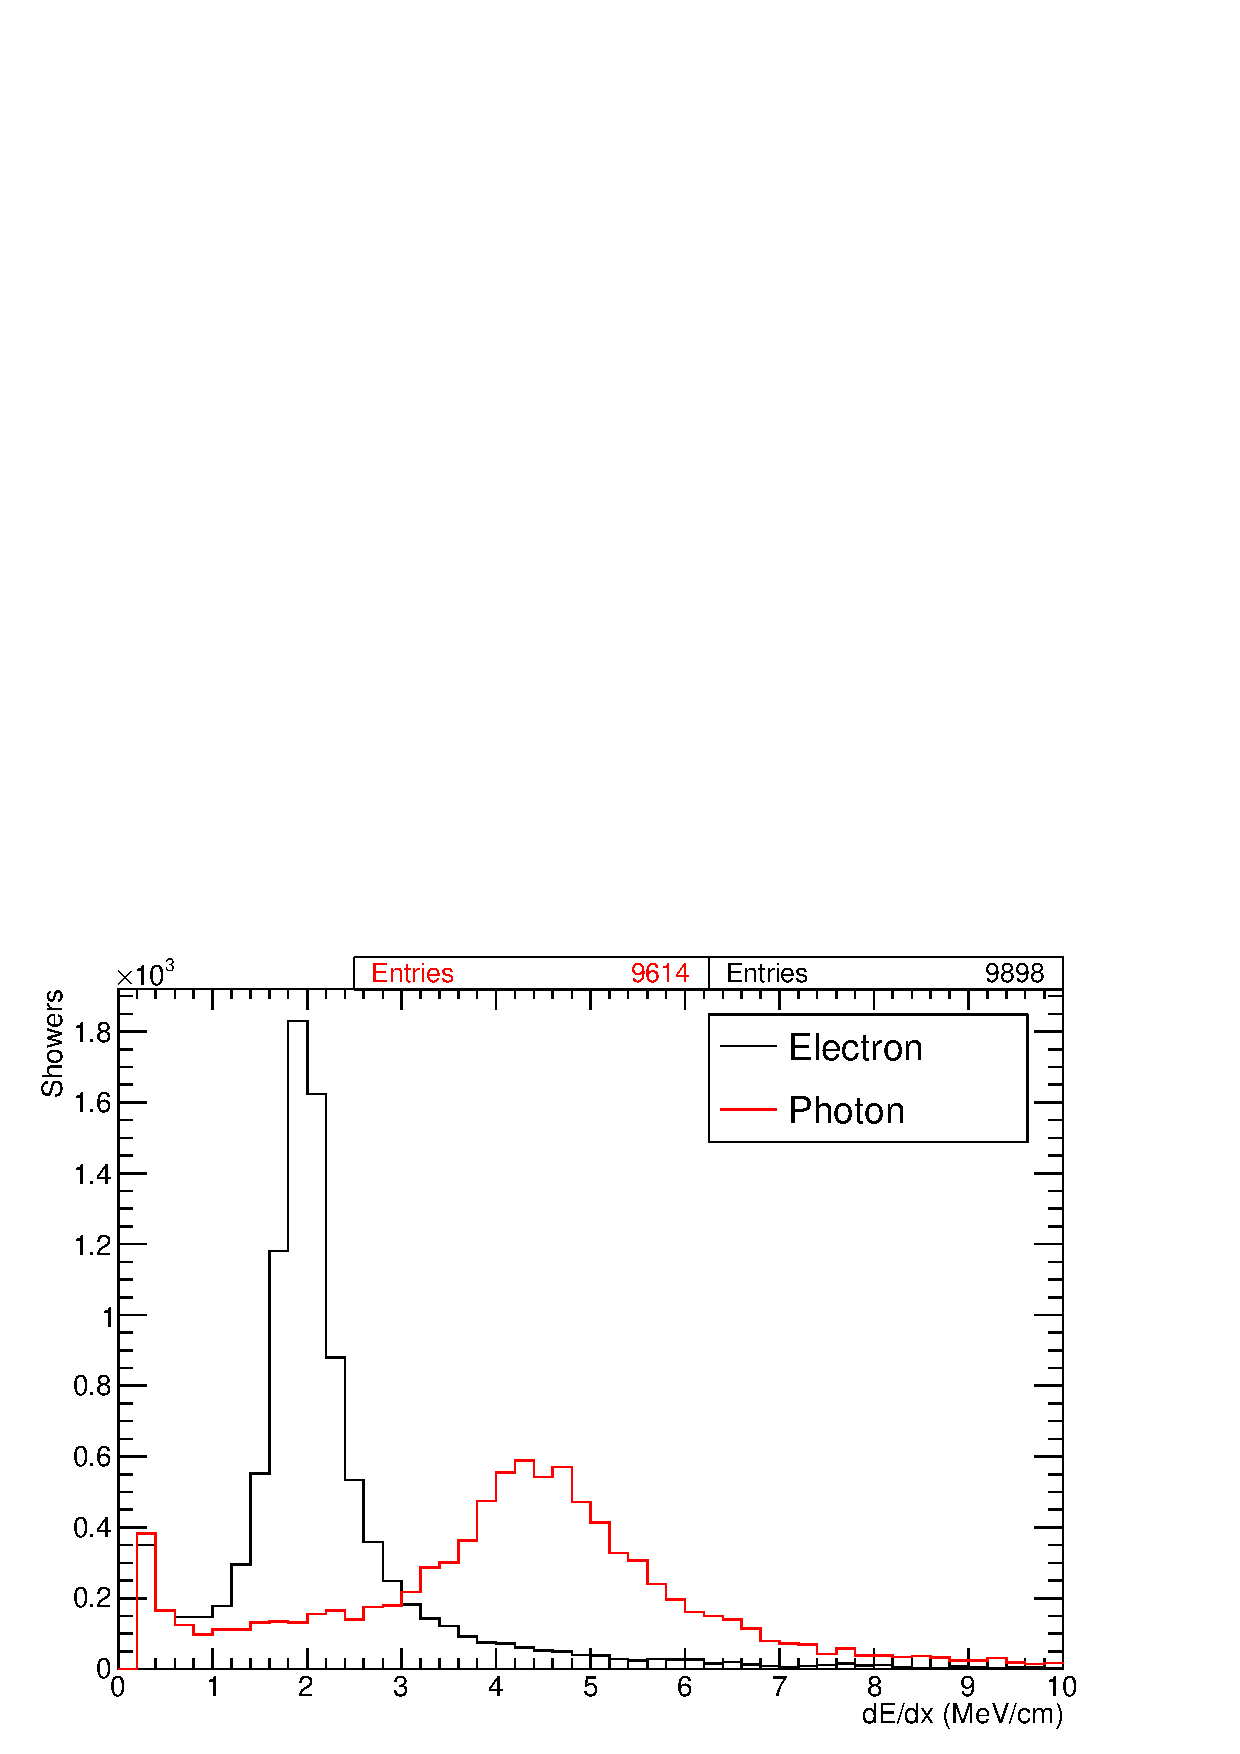
\includegraphics[width=0.9\textwidth]{ShowerdEdx.pdf}
    \caption{Shower dE/dx}
  \end{subfigure}
  %\hfill
  \begin{subfigure}[t]{0.4\linewidth}
    \centering
    \includegraphics[width=0.9\textwidth]{ShowerEnergy.pdf}
    \caption{Shower energy}
  \end{subfigure}
  %\vfill
  \begin{subfigure}[t]{0.4\linewidth}
    \centering
    \includegraphics[width=0.9\textwidth]{NHitsPerShowerWire.pdf}
    \caption{Number of hits per shower wire}
  \end{subfigure}
  %\hfill
  \begin{subfigure}[t]{0.4\linewidth}
    \centering
    \includegraphics[width=0.9\textwidth]{ShowerLength.pdf}
    \caption{Shower length}
  \end{subfigure}
  %\vfill
  \begin{subfigure}[t]{0.4\linewidth}
    \centering
    \includegraphics[width=0.9\textwidth]{ShowerMaximum.pdf}
    \caption{Shower maximum}
  \end{subfigure}
  %\hfill
  \begin{subfigure}[t]{0.4\linewidth}
    \centering
    \includegraphics[width=0.9\textwidth]{ShowerStartEventVertexX.pdf}
    \caption{Displacement of shower start ($x$-direction)}
  \end{subfigure}
  %\vfill
  \caption[MVA input variables related to information about the highest energy shower in the event for the DUNE far detector $\nu_e$CC analysis.]{MVA input variables related to information about the highest energy shower in the event for the DUNE far detector $\nu_e$CC analysis.}
  \label{fig:FDMVAShowerVariables}
\end{figure}
\begin{figure}\ContinuedFloat
  \centering
  \begin{subfigure}[t]{0.4\linewidth}
    \centering
    \includegraphics[width=0.9\textwidth]{ShowerStartEventVertexY.pdf}
    \caption{Displacement of shower start ($y$-direction)}
  \end{subfigure}
  %\hfill
  \begin{subfigure}[t]{0.4\linewidth}
    \centering
    \includegraphics[width=0.9\textwidth]{ShowerStartEventVertexZ.pdf}
    \caption{Displacement of shower start ($z$-direction)}
  \end{subfigure}
  %\vfill
  \begin{subfigure}[t]{0.4\linewidth}
    \centering
    \includegraphics[width=0.9\textwidth]{ShowerCosX.pdf}
    \caption{Shower angle ($x$-direction)}
  \end{subfigure}
  %\hfill
  \begin{subfigure}[t]{0.4\linewidth}
    \centering
    \includegraphics[width=0.9\textwidth]{ShowerCosY.pdf}
    \caption{Shower angle ($y$-direction)}
  \end{subfigure}
  %\vfill
  \begin{subfigure}[t]{0.4\linewidth}
    \centering
    \includegraphics[width=0.9\textwidth]{ShowerCosZ.pdf}
    \caption{Shower angle ($z$-direction)}
  \end{subfigure}
  %\hfill
  \caption[]{MVA input variables related to information about the highest energy shower in the event for the DUNE far detector $\nu_e$CC analysis.}
  \label{fig:FDMVAShowerVariables}
\end{figure}
